\documentclass[a4paper,leqno,10pt]{article}
\usepackage[utf8]{inputenc}
% \usepackage{lmodern}
\usepackage{OldStandard}
\usepackage{microtype}
\usepackage[inline]{enumitem}

\usepackage{siunitx}
\usepackage{multirow}
\usepackage{subcaption}

\usepackage[english]{babel}
\usepackage[autostyle, english=british]{csquotes}
\MakeOuterQuote{"}

\usepackage{commath}
\usepackage{amsmath}
\usepackage{amsthm}
\usepackage{amssymb}
\usepackage{mathtools}

\usepackage{pgfplots}
\pgfplotsset{compat=1.11}
\usepgfplotslibrary{fillbetween}
\usetikzlibrary{patterns}
\usetikzlibrary{arrows}

\usepackage{hyperref}

\usepackage[margin=1in]{geometry}
\usepackage{changepage}
\usepackage{titlesec}
\titleformat{\section}{\normalfont\Large\bfseries\centering}{Section~\thesection:}{1em}{}

\usepackage[framemethod=tikz]{mdframed}

\def\signed #1{{\leavevmode\unskip\nobreak\hfil\penalty50\hskip2em
  \hbox{}\nobreak\hfil(#1)%
  \parfillskip=0pt \finalhyphendemerits=0 \endgraf}}
\newsavebox\mybox
\newenvironment{aquote}[1]
  {\savebox\mybox{#1}\begin{quote}}
  {\signed{\usebox\mybox}\end{quote}}

% Augmented matrices.
\makeatletter
\renewcommand*\env@matrix[1][*\c@MaxMatrixCols c]{%
  \hskip -\arraycolsep
  \let\@ifnextchar\new@ifnextchar
  \array{#1}}
\makeatother

%--------grstep
% For denoting a Gauss' reduction step.
% Use as: \grstep{\rho_1+\rho_3} or \grstep[2\rho_5 \\ 3\rho_6]{\rho_1+\rho_3}
\newcommand{\grstep}[2][\relax]{%
   \ensuremath{\mathrel{
       {\mathop{\longrightarrow}\limits^{#2\mathstrut}_{
                                     \begin{subarray}{l} #1 \end{subarray}}}}}}
\newcommand{\swap}{\leftrightarrow}

\makeatletter
\newtheoremstyle{exercise}% name of the style to be used
{5pt}% measure of space to leave above the theorem. E.g.: 3pt
{3pt}% measure of space to leave below the theorem. E.g.: 3pt
{\rm}% name of font to use in the body of the theorem
{}% measure of space to indent
{\large\bf}% name of head font
{.}% punctuation between head and body
{\newline}% space after theorem head; " " = normal interword space
{\thmname{#1}\thmnumber{ #2}\thmnote{: #3}}
\makeatother

\theoremstyle{exercise}
\newtheorem{Exercise}{Exercise}
\newenvironment{exercise}
  {\begin{mdframed}\begin{Exercise}}
  {\end{Exercise}\end{mdframed}}

\theoremstyle{plain}
\newtheorem*{thm}{Theorem}
\newtheorem*{lem}{Lemma}
\theoremstyle{definition}
\newtheorem*{defn}{Definition}
\newtheorem*{ex}{Example}
\newtheorem*{axiom}{Axiom}
\theoremstyle{remark}
\newtheorem*{rem}{Remark}
\AtEndEnvironment{rem}{\hfill$\blacksquare$}%

\newcommand{\df}{\textbf}
\newcommand{\T}{\mathrm{T}}
\newcommand{\F}{\mathrm{F}}
\newcommand{\IndSet}{\mathbf{I}}
\DeclareMathOperator{\cis}{cis}
\DeclareMathOperator{\arcsec}{arcsec}
\renewcommand\vec{\mathbf}

\renewcommand{\theequation}{N\arabic{equation}}

\title{Level Three Conic Sections\\---\\Notes and solutions}
\author{Alex Elzenaar}
\date{\today}

\begin{document}
\setcounter{tocdepth}{1}

\begin{titlepage}
  \maketitle
  \begin{center}
    
\includegraphics[width=0.4\textwidth]{icecream}

    \vspace{2em}

    \begin{minipage}{\dimexpr\textwidth-4cm}
      \begin{aquote}{Grothendieck}\slshape
        The first analogy that came to my mind is of immersing the nut in some softening liquid, and why not simply water? From time to time you rub so the liquid penetrates better, and otherwise you let time pass. The shell becomes more flexible through weeks and months—when the time is ripe, hand pressure is enough, the shell opens like a perfectly ripened avocado! A different image came to me a few weeks ago. The unknown thing to be known appeared to me as some stretch of earth or hard marl, resisting penetration... the sea advances insensibly in silence, nothing seems to happen, nothing moves, the water is so far off you hardly hear it... yet it finally surrounds the resistant substance.
      \end{aquote}
    \end{minipage}
  \end{center}
  \thispagestyle{empty}
\end{titlepage}
\pagenumbering{arabic}

\tableofcontents
\section*{Preface}
This is a set of notes and outlines of solutions to the various exercises in the conic section notes.

\titleformat{\section}{\clearpage\titlerule[0.8pt]\vspace{0.5ex}\normalfont\Large\bfseries\centering}{Notes on Section~\thesection:}{1em}{}[{\titlerule[0.8pt]}]
\let\oldsection\section
\renewcommand\section{\clearpage\oldsection}
\setcounter{section}{2}\addtocounter{section}{-1}
\section{Basic results}

\begin{exercise}[Polar form]
  Show that, if $ X $ is on the directrix of a conic such that $ OX \perp \ell $, then the polar equation of the
  conic with respect to this axis and origin $ O $ is
  \begin{displaymath}
    \frac{l}{r} = 1 + \varepsilon \cos \theta.
  \end{displaymath}
  Conclude that:
  \begin{enumerate}
    \item Every conic is symmetric with respect to $ OX $.
    \item The ellipse is a closed and bounded curve (i.e. it does not extend towards infinity).
    \item The parabola is unbounded, but is connected.
    \item The hyperbola consists of two seperate branches, each extending to infinity, given by $ -\alpha < \theta < \alpha $
          and $ \alpha < \theta < 2\pi - \alpha $ (where $ \alpha = \arcsec(-\varepsilon) $).
  \end{enumerate}
\end{exercise}

Before answering this, I do need to conceed that at this stage we have no good definition for a closed curve, or a connected curve, or
for a branch/component of a curve. However, the curves we deal with are so simple that we can say that:
\begin{itemize}
  \item A closed curve is one which is periodic in $ \theta $.
  \item A component/branch of a curve is a set of points on the curve such that (1) each point in the set
        corresponds to a value of $ \theta $ taken from some open interval $ (a,b) $; and (2) each point corresponding
        to a value of $\theta $ from the interval is on the curve and has a finite radius.
  \item A connected curve is one which consists of a single component.
\end{itemize}
A fairly general and accessible version (restricted to curves in the real plane) can be found in books on multivariate calculus and/or the
geometry of curves; see for example the first couple of chapters of do Carmo.\footnote{\emph{Differential geometry of curves and surfaces}.}
However, the `proper' generalisation comes from topology: see for example Munkres (\S 23--24).

Let us consider the following diagram.
\begin{center}
  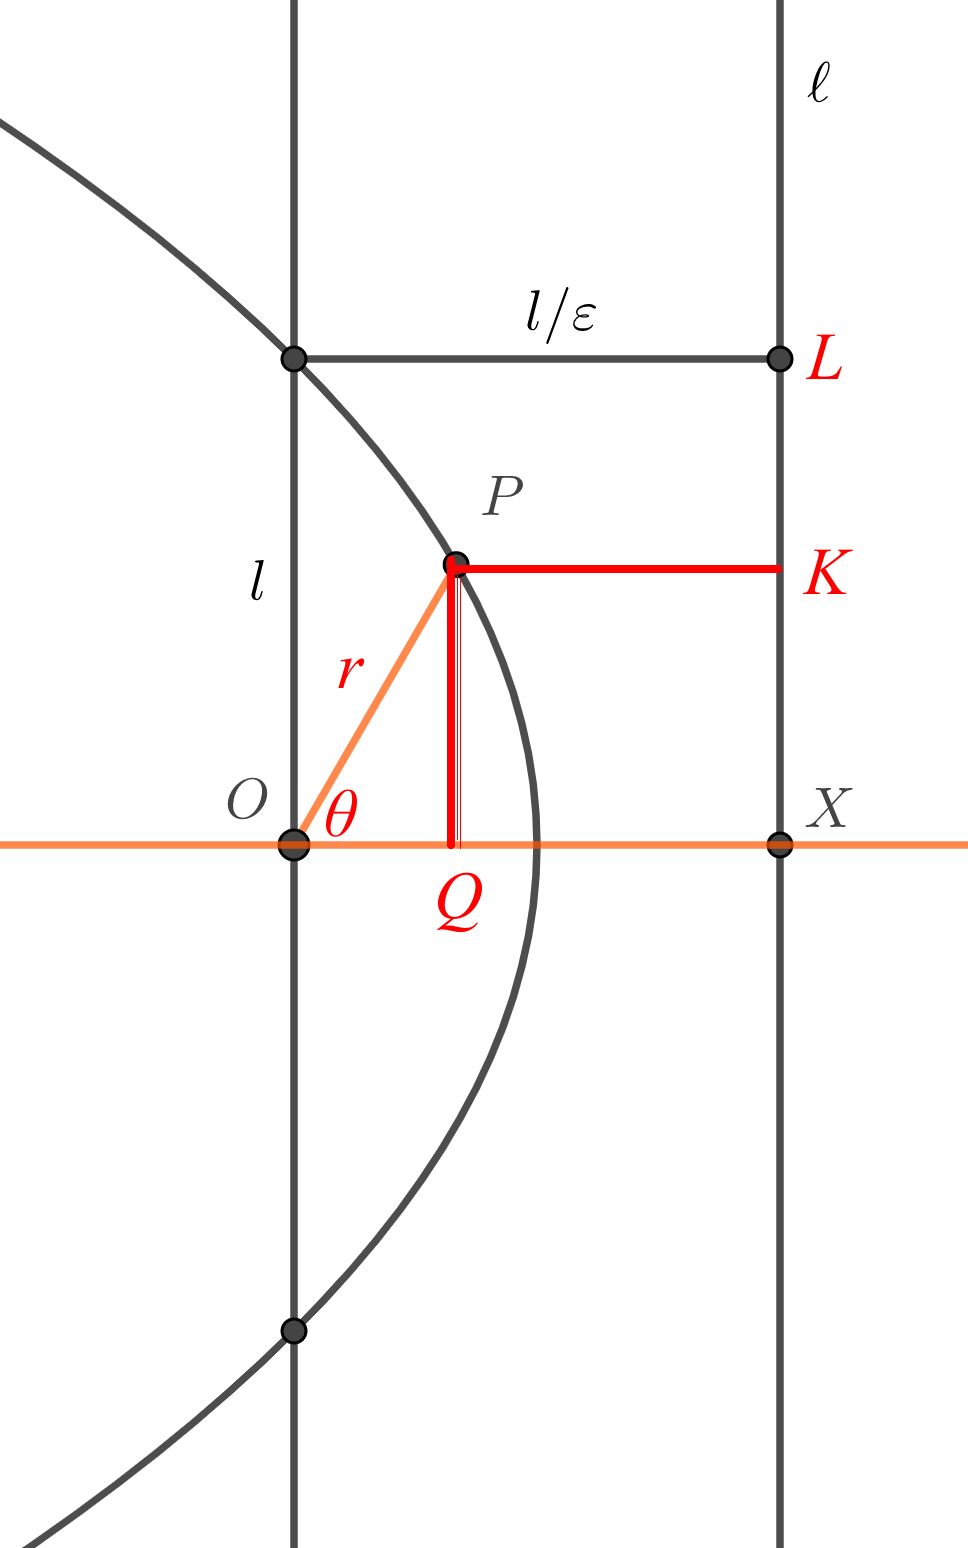
\includegraphics[width=0.3\textwidth]{solutions1}
\end{center}
We have the following: $ \abs{OQ} = \abs{OX} - \abs{QX} $. But $ \abs{OQ} = r\cos \theta $, $ \abs{OX} = e/\varepsilon $, and $ \abs{QX} = \abs{PK} $;
thus $ r \cos \theta = l/\varepsilon - \abs{PK} $. But since $ P $ is on the conic, $ \varepsilon = \abs{OP}/\abs{PK} = r/\abs{PK} $;
hence $ r \cos \theta = l/\varepsilon - r/\varepsilon $ and thus $ l/r = 1 - \varepsilon \cos \theta $.

For (1), we need to check that the graph is symmetric about $ OX $; this ray is our polar axis, and so we just need to check that $ (r, \theta) $
is on $ \mathcal{C} $ iff $ (r, -\theta) $ is on the curve. But $ \cos \theta = \cos (-\theta) $, which is sufficient.

For (2), we need to do some work with inequalities. From the polar equation, $ r = \frac{l}{1 + \varepsilon \cos \theta} $;
so we need to show that this fraction is bounded above (i.e. given any eccentricity $ \varepsilon $ and any length $ l $ then there exists some $ K $ --- which
depends on $ \varepsilon $ and $ l $ --- such that $ \abs{r} < K $ for all possible $ \theta $). Let us therefore fix a given eccentricity $ \varepsilon $. Since
the conic is an ellipse, we have $ 0 \leq \varepsilon < 1 $.

Since $ \varepsilon $ is real, there exists some positive $ \kappa $ satisfying $ \varepsilon < \kappa < 1 $.\footnote{We need \df{completeness} here.}
Hence we have that $ 0 < \varepsilon < \kappa $, and thus $ -\kappa < -\varepsilon < 0 $; so $ 1 - \kappa < 1 - \varepsilon < 1 $,
and thus $ 1 + \varepsilon \cos \theta \geq 1 - \varepsilon > 1 - \kappa $.

From this, we have that $ \frac{1}{1 - \varepsilon \cos \theta} < \frac{1}{1 - \kappa} $, and hence $ r < \frac{l}{1 - \kappa} < \infty $.

Further, $ 1 + \varepsilon \cos \theta \leq 1 + \varepsilon < 2 $, so $ \frac{1}{2} < \frac{1}{1 + \varepsilon \cos \theta} $ and
thus $ \frac{l}{2} < r $. Combining our two $ r$-involving inequalities, we obtain

\begin{displaymath}
  \frac{l}{2} < r < \frac{l}{1 - \kappa};
\end{displaymath}
so $ r $ (and thus the curve) is bounded. The closedness of the curve is trivial, since $ r $ is periodic (with period dividing $ 2\pi $.)

For (3), we need to show the parabola $ r = \frac{l}{1 + \cos \theta} $ is unbounded (note $ \varepsilon = 1 $). But this is clearly
true, for if $ \theta \to \pi $ then $ r \to \infty $. The parabola is connected, since $ \theta = \pi $ is the only discontinuity,
and the curve is periodic otherwise: to see this more clearly, let $ \theta $ vary from $ -\pi $ to $ \pi $; the result covers the entire
parabola, and is only discontinuous at the endpoints.

Now for (4) we proceed similarly to (3); the curve is periodic with period $ 2\pi $, and $ r \to \infty $ precisely
when $ 1 + \varepsilon \cos \theta \to 0 $; this latter phenomenon occurs when $ \cos \theta = -1/\varepsilon $,
which is equivalent to $ \sec \theta = -\varepsilon $. Fix $ \alpha = \arcsec(-\varepsilon) $; then all of $ -\alpha $, $ \alpha $,
and $ 2\pi - \alpha $ satisfy $ \sec(\theta) = -\varepsilon $, and these three points are the only points in the interval $ [-\alpha, 2\pi - \alpha] $
which satisfy this. If $ \theta $ ranges over this interval we cover the entire curve, and $ r \to \infty $ only at the endpoints and
at $ \theta = \alpha $. Hence the curve is in two components (since it is continuous everywhere in the interval except these three points),
and tends to infinity at the claimed angles.

\begin{exercise}[Rectangular form]\label{exercise:rectangular}
  By squaring the polar form equation, show that the Cartesian equation for a conic, taking suitable axes and origin, is
  \begin{displaymath}
    x^2 + y^2 = (l - \varepsilon x)^2.
  \end{displaymath}
  \begin{enumerate}
    \item If $ \varepsilon \neq 1 $, and a suitable origin is chosen, show that the conic equation can be written in the form
          \begin{displaymath}
            \frac{x^2}{a^2} \pm \frac{y^2}{b^2} = 1
          \end{displaymath}
          for some real numbers $ a $ and $ b $. The new location of the origin is called the \df{centre} of the conic. Conclude that:
          \begin{enumerate}
            \item Both the ellipse and hyperbola are symmetric across both Cartesian axes.
            \item For an ellipse, the values $ 2a $ and $ 2b $ are the lengths of the chords through the origin along the $ x$- and $ y$-axes respectively. (The
                  longer of these is called the \df{major axis}, and the shorter the \df{minor axis}.)
            \item The two branches of a hyperbola lie in opposite regions formed by the two lines (\df{asymptotes})
                    \begin{displaymath}
                      \left(\frac{x}{a} - \frac{y}{b} \right)\left(\frac{x}{a} + \frac{y}{b} \right) = 0.
                    \end{displaymath}
                    The value $ 2a $ is the length of the transverse axis of the hyperbola and the value $ 2b $ is the length of the conjugate
                    axis: the two dimensions of the rectangle whose diagonals are the asymptotes and which is bounded by the hyperbola.
            \item Further, show that as $ x \to \pm\infty $, the branches of the hyperbola tend arbitrarily close to the asymptotes. (Hint: take limits.)
          \end{enumerate}
    \item If $ \varepsilon = 1 $, show that the conic equation for the parabola can be written in the form
          \begin{displaymath}
            y^2 = 2l(\frac{1}{2}l - x).
          \end{displaymath}
          By reflecting in a suitable vertical line, derive the standard form equation
          \begin{displaymath}
            y^2 = 2lx.
          \end{displaymath}
          Given this latter equation, give the coordinates of the focus, and the Cartesian equation of the directrix.
  \end{enumerate}
\end{exercise}

We will pick our origin to be $ O $, our $ x$-axis to be the ray in the direction of $ X $ (i.e. the polar axis), and the $ y$-axis to be
the line through $ O $ perpendicular to $ OX $.

To compute the rectangular form equation take $ r = l - \varepsilon r \cos \theta $, so $ r^2 = l^2 - 2l\varepsilon r \cos\theta + \varepsilon^2 r^2 \cos^2\theta $
and then (substituting) $ x^2 + y^2 = l^2 - 2l\varepsilon x + \varepsilon^2 x^2 = (l - \varepsilon x)^2 $.

Assume $ \varepsilon \neq 1 $. Then we collect terms and complete the square:
\begin{align*}
  x^2 + y^2 = (l - \varepsilon x)^2 &\implies (1 - \varepsilon^2)x^2 + 2l\varepsilon x + y^2 = l^2\\
                                    &\implies x^2 + \frac{2l\varepsilon}{1 - \varepsilon^2} + \frac{y^2}{1 - \varepsilon^2} = \frac{l^2}{1 - \varepsilon^2}\\
                                    &\implies \left(x + \frac{l\varepsilon}{1 - \varepsilon^2}\right)^2 - \frac{l^2 \varepsilon^2}{(1 - \varepsilon^2)^2} + \frac{y^2}{1 - \varepsilon^2} = \frac{l^2}{1 - \varepsilon^2}\\
                                    &\implies \left(x + \frac{l\varepsilon}{1 - \varepsilon^2}\right)^2 + \frac{y^2}{1 - \varepsilon^2} = \frac{l^2}{(1 - \varepsilon^2)^2}.
\end{align*}

\begin{rem}
  I will take some liberties here with regard to choosing $ b $. In particular, we 'want' $ b $ to be such that $ b^2 $ is negative when we have
  a hyperbola, so we should take $ b = i\beta $ (where $ \beta $ is half the length of the conjugate axis); on the other hand, it is much
  easier to interpret $ b $ as a length if it is real.

  In these notes, I will reverse this notation here and take $ b $ to be the \emph{length} which is half the $ y$-chord (for both the hyperbola and the ellipse),
  and $ \beta = ib $ to be the purely imaginary number which has the same modulus. This notation is not standard.
\end{rem}

Set $ a = \frac{l}{1 - \varepsilon^2} $, and $ \beta = \sqrt{1 - \varepsilon^2}a $ (where $ \beta $ will be be imaginary, in the case of a hyperbola).
Then set $ b = \abs{\beta} $.

Let us make a change of coordinates, sending $ (x,y) \mapsto (x',y') = (x - \varepsilon a) $; then our equation becomes
\begin{equation}\label{eqn:generalconic}
  \frac{{x'}^2}{a^2} \pm \frac{{y'}^2}{b^2} = 1
\end{equation}
where the sign $ \pm $ is the same as the sign of $ 1 - \varepsilon^2 $; more precisely, our equation becomes
\begin{equation}\label{eqn:generalconic}
  \frac{{x'}^2}{a^2} + \frac{{y'}^2}{\beta^2} = 1
\end{equation}
but the former is more usual.

Note also that $ l = \frac{\beta^2}{a} $, in this coordinate system.

If $ (x,y) $ satisfies the equation \ref{eqn:generalconic}, by the properties of squaring all four sign permutations of $ (\pm x , \pm y) $ satisfy it as
well; so the curve is indeed symmetric across both axes.

Now, suppose we have an ellipse; so the sign in the equation is $ + $. The $ x$-intercepts of the curve are $ x = \pm a $, so the chord along
the $ x$-axis has length $ 2a $. By the same reasoning, the $ y$-intercepts are $ y = \pm b $, so the $ y$-axis chord has length $ 2b $.

Now let us consider the case of a hyperbola. We have shifted our origin, and so we need to compute a new polar form, depending on $ a $
and $ b $. Since $ r^2 = x^2 + y^2 $ and $ \tan \theta = \frac{y}{x} $, we have $ r^2 = x^2(1 + \tan^2 \theta) = x^2 \sec^2 \theta $.
Substituting:
\begin{displaymath}
  1 = \frac{x^2}{a^2} - \frac{y^2}{b^2} = \frac{r^2}{a^2\sec^2 \theta} - \frac{r^2 \tan^2 \theta}{b^2\sec^2 \theta} = r^2 \left( \frac{b^2 - a^2 \tan^2 \theta}{a^2b^2 \sec^2\theta} \right)
\end{displaymath}
and hence
\begin{equation}
  r = \frac{ab \abs{\sec \theta}}{\sqrt{b^2 - a^2 \tan^2 \theta}}
\end{equation}
is our new polar form (let us call it \df{central polar form}; in these notes, we will call the polar form from exercise 1 the \df{focus polar form}).

\begin{rem}
  Let us translate this into the use of imaginary axes, so we can use the same formula for the ellipse as well. We have the following:
  \begin{displaymath}
    1 = \frac{x^2}{a^2} + \frac{y^2}{\beta^2} = \frac{r^2}{a^2\sec^2 \theta} + \frac{r^2 \tan^2 \theta}{\beta^2\sec^2 \theta} = r^2 \left( \frac{\beta^2 + a^2 \tan^2 \theta}{a^2\beta^2 \sec^2\theta} \right)
  \end{displaymath}
  and hence
  \begin{equation}
    r = \abs{\frac{ab \sec \theta}{\sqrt{\beta^2 + a^2 \tan^2 \theta}}} = \frac{ab \abs{\sec \theta}}{\sqrt{\abs{\beta^2 + a^2 \tan^2 \theta}}}.
  \end{equation}

  We can now ``nicely'' write down an equation for $ \varepsilon $ in terms of $ a $ and $ \beta $: since $ a = \frac{l}{1 - \varepsilon^2} $
  and $ l = \frac{\beta^2}{a} $, we have that $ \varepsilon^2 = \frac{a^2 - \beta^2}{a^2} $; this becomes $ \varepsilon^2 = \frac{a^2 + b^2}{a^2} $
  for an ellipse, and $ \varepsilon^2 = \frac{a^2 - b^2}{a^2} $ for a hyperbola. (This use of imaginary axes for the hyperbola thus wraps up the
  two different formulae for the eccentricity into a single formula, which is nice.)
\end{rem}

Since we have only performed a translation, our curve is still in two disconnected branches. The equation for $ r $ is periodic with period $ 2\pi $,
and is undefined precisely when $ b^2 - a^2 \tan^2 \theta \leq 0 $. The `boundaries' of this area are thus the bounding lines of the hyperbola, and
are the lines described by $ b^2 - a^2 \tan^2 \theta = 0 $, or $ \tan \theta = \pm \frac{b}{a} $; in other words, $ y = \pm \frac{b}{a}x $.

We can now give the dimensions for the axes of the hyperbola. The $ x$-intercepts of the hyperbola, as for the ellipse, are $ x = \pm a $. Thus the
four corners of the rectangle are $ (a, b) $, $ (-a, b) $, $ (a, -b) $, and $ (-a, -b) $. Thus the two side lengths of the rectangle, as claimed,
are $ 2a $ (in the $ x$-direction) and $ 2b $ (in the $ y$-direction). [Note, in this situation we take $ b $ to be real, not imaginary.]

Finally, as $ x \to \infty $, we need to show that the curve becomes arbitrarily close to the asymptotes. Indeed, we can easily show
that $ \od{y}{x} = \frac{x b^2}{y a^2} $. Consider the portion of the hyperbola where $ x > 0 $ and $ y > 0 $. Here,
\begin{displaymath}
  y = b\sqrt{\frac{x^2}{a^2} - 1}
\end{displaymath}
and so the equation of the tangent to the curve at $ (x_0, y_0) $ is
\begin{displaymath}
  y = \frac{x_0 b^2}{y_0 a^2} (x - x_0) + y_0
    = \frac{x_0 b}{a^2\sqrt{\frac{x_0^2}{a^2} - 1}} x - \frac{x_0^2 b}{a^2\sqrt{\frac{x_0^2}{a^2} - 1}} + b\sqrt{\frac{x_0^2}{a^2} - 1}.
\end{displaymath}
The slope of the tangent line, as $ x_0 \to \infty $, is
\begin{displaymath}
 \frac{x_0 b}{a^2\sqrt{\frac{x_0^2}{a^2} - 1}} = \frac{b}{a^2\sqrt{\frac{1}{a^2} - \frac{1}{x_0^2}}} \to \frac{b}{a^2\sqrt{\frac{1}{a^2} - 0}} = \frac{b}{a}.
\end{displaymath}
Further, the $ y$-intercept becomes
\begin{displaymath}
  -\frac{x_0^2 b}{a^2\sqrt{\frac{x_0^2}{a^2} - 1}} + b\sqrt{\frac{x_0^2}{a^2} - 1} = \frac{ba^2(\frac{x_0^2}{a^2} - 1)-x_0^2 b}{a^2\sqrt{\frac{x_0^2}{a^2} - 1}}
    = \frac{- ba^2}{a^2\sqrt{\frac{x_0^2}{a^2} - 1}}
    \to 0
\end{displaymath}
when $ x_0 \to \infty $.

Thus the tangent line of the curve approaches $ y = \frac{b}{a} x $ as $ x \to \infty $, and hence the curve itself approaches this line. We can perform similar
calculations for the various cases where $ x < 0 $ or $ y < 0 $ (or both).

For the parabola, since $ \varepsilon = 1 $, we obtain $ x^2 + y^2 = (l - x)^2 = l^2 - 2lx + x^2 $, and so $ y^2 = 2l(\frac{1}{2}l - x) $.
If we reflect in the line $ x = l/4 $, then we map
\begin{displaymath}
  (x,y) \to (-(x - l/4) + l/4, y) = (l/2 - x, y)
\end{displaymath}
and our equation becomes
\begin{displaymath}
  y^2 = 2l\left(\frac{l}{2} - \frac{l}{2} + x \right) = 2lx.
\end{displaymath}

We obtained the equation $ y^2 = 2l(\frac{1}{2}l - x) $ using the focus polar form, and so in that form the focus was $ (0,0) $. In doing
our reflection, we mapped $ (0,0) \to (l/2,0) $; hence this is the location of the focus. In other words, if $ y^2 = 4ax $, then $ 2l = 4a $
and $ a = l/2 $; so $ (a,0) $ is the focus. The directrix of the original form was located at $ x = l/\varepsilon = l $; after the transformation,
it is located at $ x = -l/2 $, or (if we write the equation as $ y^2 = 4ax $) it is located at $ x = -a $. (These results suggest that $ y^2 = 4ax $
is the most natural form for the equation of the parabola.)

\begin{exercise}[Parametric form]
  Show that:
  \begin{enumerate}
    \item The ellipse $ x^2/a^2 + y^2/b^2 = 1 $ is parameterised by $ (a \cos t, b \sin t) $ for $ 0 \leq t < 2\pi $.
    \item The parabola $ y^2 = 2lx $ is parameterised by $ (2lt^2, 2lt) $.
    \item The hyperbola $ x^2/a^2 - y^2/b^2 = 1 $ is parameterised by $ (a \sec t, b \tan t) $ for $ 0 \leq t < 2\pi $.
  \end{enumerate}
  Illustrate these parameterisations with a suitable computer program (e.g. Geogebra, or your favourite programming language).
\end{exercise}

Consider the ellipse case. We need to show two things:
\renewcommand{\labelenumi}{\Roman{enumi}.}
\begin{enumerate}
  \item That each point of the form $ (a \cos t, b \sin t) $ lies on the ellipse.
  \item That for each point $(x,y)$ on the ellipse there exists some unique $ t $ lying in the range $ 0 \leq t < 2\pi $
        such that $ (x,y) = (a \cos t, b \sin t) $.
\end{enumerate}

Point I is easy: $ (a \cos t)^2/a^2 + (b \sin t)^2/b^2 = \cos^2 t + \sin^2 t = 1 $, so each such point is indeed on the ellipse.

Now, suppose $ (x,y) $ lies on the ellipse. Let us begin by finding all $ t $ such that $ a \cos t = x $; indeed,
$ \cos t = x/a $, and (by our earlier results) we know that $ \abs{x} \leq \abs{a} $ so there exists some $ t_0 $ in the given range
such that $ \cos t_0 = x/a $; further, $ 2\pi - t_0 $ is the only other point in the range which might satisfy this equation.

Let us now consider $ \sin t_0 $ and $ \sin (2\pi - t_0) $. We have $ x^2/a^2 + y^2/b^2 = 1 $, so $ \cos^2 t_0 + y^2/b^2 = 1 $. It
follows that $ 1 - \sin^2 t_0 + y^2/b^2 = 1 $, and hence that $ \sin^2 t_0 = y^2/b^2 $; so $ \sin t_0 = \pm y/b $.

Suppose that $ \sin t_0 = -y/b $. Then $ \sin (2\pi - t_0) = -\sin(t_0) $ (by standard properties of the sine function),
and so $ \sin(2\pi - t_0) = y/b $; thus $ y = b\sin(2\pi - t_0) $ and $ x = a\cos(2\pi - t_0) $, $ t = 2\pi - t_0 $ is the
only substitution such that both $ y = b\sin t $ and $ x = a\cos t $ work.

It remains to show that if $ \sin t_0 = y/b $ then $ \sin (2\pi - t_0) \neq y/b $ (for if both held, then we wouldn't have
a unique value for $ t $: both $ t_0 $ and $ 2\pi - t_0 $ would work). But by the same reasoning as above, $ \sin t_0 = y/b $
implies $ \sin (2\pi - t_0) = -y/b \neq y/b $; so if $ \sin t_0 = y/b $ then the substitution $ t = t_0 $ is the unique parameter
giving the point $ (x,y) $.

The same process works for both the hyperbola and the ellipse.

\begin{exercise}[Focii of rectangular conics]
  Given the equation
  \begin{displaymath}
    \frac{x^2}{a^2} \pm \frac{y^2}{b^2} = 1,
  \end{displaymath}
  compute the coordinates of the focus, equation of the directrix, and eccentricity of the conic. Hence show that
  ellipses and hyperbolae have two focii and two directrices each. Where is the directrix of a circle?

  Show that the following two properties can be used as alternative definitions for the ellipse and hyperbola:
  \begin{enumerate}[label={AP\arabic*}.]
    \item Show that the ellipse with focii $ O_1 $ and $ O_2 $ is the locus of all points $ P $
          such that $ d(O_1, P) + d(P, O_2) = R $ for some constant $ R $. Give $ R $ in terms of $ a $ and $ b $.
    \item Show that the hyperbola with focii $ O_1 $ and $ O_2 $ is the locus of all points $ P $
          such that $ d(O_1, P) - d(P, O_2) = R $ for some constant $ R $. Give $ R $ in terms of $ a $ and $ b $.
  \end{enumerate}

  As an application of this definition, we will derive the `reflection property' of the ellipse.
  \begin{enumerate}
    \item Suppose $ O_1 $ and $ O_2 $ are on the same side of a line $ \ell $. Show that the shortest path from $ O_1 $
          to $ O_2 $ which touches the line $ \ell $ is the broken line $ O_1XO_2 $, where $ X $ is on $ \ell $ and
          the angles between $ O_1 X $ and $ \ell $ and between $ X O_2 $ and $ \ell $ are equal. (Hint: you can do this
          with calculus, but that would be like killing a fly with a sledgehammer.)
    \item Show that, if $ O_1 $ and $ O_2 $ are two focii of an ellipse and $ X $ is any point on the ellipse, then the broken line $ O_1 X O_2 $
          makes equal angles with the tangent line of the ellipse at $ X $. (Hint: show that this broken line is the shortest path from $ O_1 $ to $ O_2 $
          that touches the tangent line at $ X $.)
    \item Thus, given the law of reflection for waves, show that if a light source is placed at $ O_1 $ then every ray from the source
          will arrive at $ O_2 $ at precisely the same time.
    \item Derive some result of this kind for parabolae by treating a parabola as an ellipse with one focus `at infinity'. Suggest an
          application of this property related to, say, torches.
  \end{enumerate}
\end{exercise}

We saw in exercise 2 that $ l = \frac{\beta^2}{a} $ and $ \varepsilon^2 = \frac{a^2 - \beta^2}{a^2} $ (where, again, $ \beta = b $ for an ellipse
and $ \beta = ib $ for a hyperbola). When origin is at the focus, the directrix was $ x = l/\varepsilon $; when we put the equation into the
normal rectangular form, we performed the transformation $ (x,y) \mapsto (x - \varepsilon a, y) $ and so the focus is now at $ (-\varepsilon a, 0) $;
if $ c = \varepsilon a $ then $ c^2 = \varepsilon^2 a^2 = a^2 - \beta^2 $; thus the focii lie at $ (\pm c, 0) = (\pm(a^2 - \beta^2), 0) $. The
directrix is now at
\begin{align*}
  x &= l/\varepsilon - \varepsilon a = \frac{\beta^2}{a\varepsilon} - \varepsilon a = \frac{\beta^2 - \varepsilon^2 a^2}{\varepsilon a}
     = \frac{2\beta^2 - a^2}{\varepsilon a}\\
  x^2 &= \frac{(2\beta^2 - a^2)^2}{a^2 - \beta^2}.
\end{align*}

For a circle, $ \beta = a $. Hence the directrix will be ``at infinity'' in the sense that it is undefined but that $ x \to \infty $ in the above
calculation as $ \beta \to a $.

(Note that we don't actually need to do any calculations to show that ellipses and hyperbolae must have two focii and two directrices, because it
follows immediately from the fact that the figures are symmetric about the $ y$-axis and so the reflections of the initial focus and directrix from
the definition must also generate the same conic.)

We will now prove the `string-and-stakes' definitions for the ellipse.\footnote{For an explanation of the name `string-and-stakes',
see \url{https://www.youtube.com/watch?v=Et3OdzEGX_w}.}

Suppose $ O_1 $ and $ O_2 $ are two points, and that $ R $ is some positive number. Let $ \mathcal{F} $ be the locus of all points $ P $
satisfying the relation $ d(P,O_1) + d(P,O_2) = R $. We want to do some coordinate geometry, so we need to pick a coordinate system; we will
chose the origin to be the midpoint $ O = m(O_1, O_2) $ and then, setting $ c = d(O_1, O) = d(O_2, O) $, we will place $ O_1 $ and $ O_2 $
on the $ x$-axis at $ O_1 = (-c, 0) $ and $ O_2 = (c,0) $.

Let $ P = (x,y) $ satisfy the given relation; then $ R = \sqrt{(x + c)^2 + y^2} + \sqrt{(x - c)^2 + y^2} $, so
\begin{align*}
  (R - \sqrt{(x - c)^2 + y^2})^2 &= x^2 + 2xc + c^2 + y^2\\
  R^2 - 2R\sqrt{(x - c)^2 + y^2} &= 4xc\\
  (x - c)^2 + y^2 &= \left(\frac{R^2 - 4xc}{2R}\right)^2\\
  x^2 - 2cx + c^2 + y^2 &= \frac{R^4 - 8cR^2x + 16c^2x^2}{4R^2}\\
  x^2 + c^2 + y^2 &=  \frac{R^2}{4} + \frac{4c^2}{R^2}x^2\\
  \frac{1 - \frac{4c^2}{R^2}}{\frac{R^2}{4} - c^2} x^2 + \frac{1}{\frac{R^2}{4} - c^2}y^2 = 1.
\end{align*}
So every such point $ P $ lies on the ellipse with $ a^2 = \frac{\frac{R^2}{4} - c^2}{1 - \frac{4c^2}{R^2}} $ and $ b^2 = \frac{R^2}{4} - c^2 $.

Further, suppose $ P = (x,y) $ lies on the ellipse. We need to show that $ R = d(O_1, P) + d(O_2, P) $; this can be done by simply running
the above calculation backwards.

A similar computation can be done for the hyperbola.

\section{Isometries}

\section{Cones}

\section{Orthogonal families of conics}

\section{Applications to physics}

\section{The intersection theorem}

\appendix
\titleformat{\section}{\clearpage\titlerule[0.8pt]\vspace{0.5ex}\normalfont\Large\bfseries\centering}{Appendix~\thesection:}{1em}{}[{\titlerule[0.8pt]}]
\section{Further reading}
See references in text, as well as:
\begin{itemize}
  \item H.S.M. Coxeter, \emph{Introduction to geometry}. John Wiley \& Sons (1961).
  \item Stephen D. Fisher, \emph{Complex variables}. Dover (1999).
  \item Robin Hartshorne, \emph{Geometry: Euclid and beyond}. Springer (2000).
  \item Keith Kendig, \emph{Conics}. Mathematical Association of America (2005).
  \item Morris Kline, \emph{Mathematics for the nonmathematician}. Dover (1985).
  \item John M. Lee, \emph{Axiomatic geometry}. American Mathematical Society (2017).
  \item George Salmon, \emph{A treatise on conic sections}. Longmans, Green (1900).
  \item George F. Simmons, \emph{Differential equations with applications and historical notes}. McGraw-Hill (1991).
  \item Marta Sved, \emph{Journey into geometries}. Mathematical Association of America (1991).
\end{itemize}

\end{document}

